\chapter[Description des rhotiques - État de l'art]{Description des rhotiques\\
\LARGE{État de l'art : \textit{R}-itage}}
\setlength{\epigraphwidth}{0.4\textwidth}
\epigraph{\href{https://www.youtube.com/watch?v=aLVMmgviTGU}{{\cjkfont 歯茎ふるえ音}} }

Les rhotiques forment un groupe complexe. Dans ce chapitre nous définissons ce que sont les rhotiques, les sons \textg{simil\textit{r}} en mentionnant les principaux membres du groupe et en résumant leur distribution dans les langues du monde selon \textcite{maddiesonPatternsSounds1984}. Nous définissons aussi ce qu'est la classe des rhotiques. Nous détaillons avec intérêt pour le reste de cette thèse des aspects de la phonétique et de la phonologie du trill, du tap et du flap. Finalement, dans ce chapitre, nous reportons des travaux typologiques sur la variation dans les rhotiques. La variation est présente au niveau de l'individu, entre les individus, au sein d'une langue, entre les langues. Pour la variation au sein d'une langue, nous donnons l'exemple du français et de l'espagnol qui sont parlés dans plusieurs régions du monde et pour lesquels la réalisation des rhotiques est variable. Finalement, nous détaillons pourquoi nous jugeons nécessaire de s'intéresser au \textg{trill} cross-linguistiquement.

%Tout d'abord, nous allons voir ce qui est généralement sous-entendu et englobé par le terme \textg{rhotique}. Cette catégorie est une classe phonologique qui doit émerger d'analyses phonologiques qui sont spécifiques à chaque langue. Nous ferons une description des principaux segments qui sont compris dans cette catégorie hétérogène.


%Une typologie des rhotiques doit paradoxalement commencer en se focalisant sur des segments \textg{simil-r} et non pas des phonèmes rhotiques. En effet, une typologie des rhotiques doit dans un premier temps comparer des éléments de la phonétique, les segments \textg{simil-r}, puis dans un second temps peut se permettre de regarder du côté de la phonologie pour observer si des régularités émergent.



\section{Représentation et caractérisation des rhotiques et des sons \textg{simil-\textit{r}}} \label{sec:similr}


Le terme \textg{rhotique} fait appel à un concept en linguistique qui peut être habituellement représenté par le \textg{r} avec la lettre minuscule <r> ou majuscule <R> et leurs dérivés. 
Bien que le terme \textg{rhotique} semble être dérivé de la lettre grec <\begin{greek}ρ\end{greek}> \parencite{wieseRepresentationRhoticsRepresentation2011}, il semble que ce terme ait émergé à la fin des années 1960 (\autoref{fig:googlengramrhotic}) avec \href{http://phonetic-blog.blogspot.com/2010/07/rhotic.html}{John Wells} qui souhaitait parler de certains accents britanniques qui conservent le \textg{r} \parencite[78--79]{wellsJohnWellsPhonetic2010,wellsSoundsInteresting2014}.
Auparavant, l'expression \textg{\textit{r}-like sounds} était plutôt utilisée pour faire référence à ces sons représentés par le <r> et <R>, comme dans \textcite[78]{maddiesonPatternsSounds1984}. Nous traduirons \textg{\textit{r}-like sounds} par \textg{sons simil-\textit{r}}.
Les essais autour de la caractérisation du comportement des rhotiques et de ce qui en fait une classe phonologique ont donné une connotation de l'ordre de la phonologie au terme de rhotique. De son côté, le terme de son \textg{simil-r} est davantage resté dans une connotation de l'ordre de la phonétique.
Malgré la terminologie, le concept de rhotique reste d'ordinaire compris à travers les membres qui le composent, on parle alors de \textg{rhotiques}. Une première définition en extension consiste à décrire les différents segments appartenant à la catégorie des rhotiques. Le concept de rhotique subsiste par le besoin des linguistes de rendre compte de l'association qui existe entre les membres de la catégorie. Nous verrons, par la suite, la définition en intention utilisant le comportement phonologique des segments, qui doivent se comporter similairement.

\begin{figure}
	\centering
	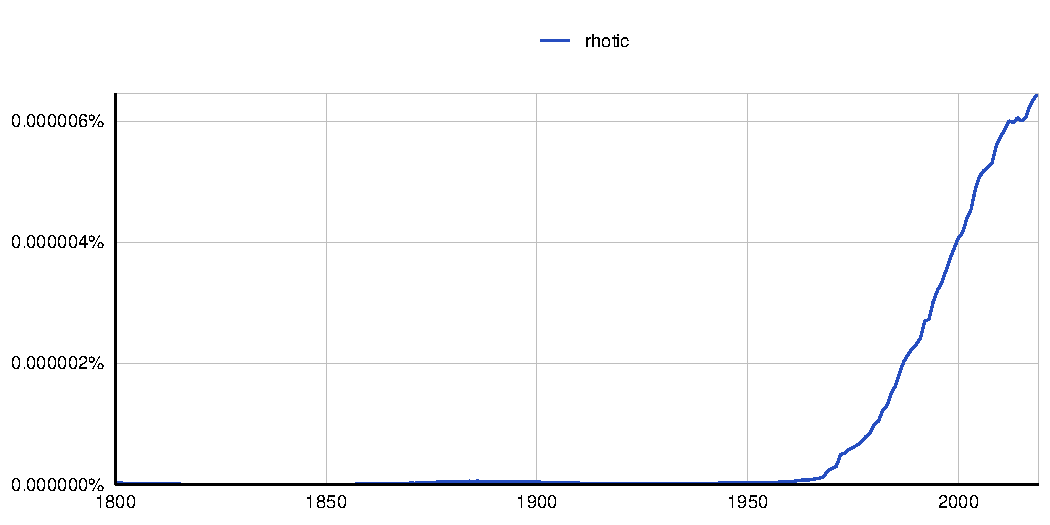
\includegraphics[width=1\linewidth]{images/google_ngram_rhotic}
	\caption[Google n-grams de \textg{rhotic}]{Fréquence de l'expression \textg{rhotic} à partir des données de Google Books en utilisant le package \texttt{ngramr} sur \texttt{RStudio} \parencite{rcoreteamLanguageEnvironmentStatistical2020}, à partir du jeu de données de Google 2019.}
	\label{fig:googlengramrhotic}
\end{figure}

\subsection{Les différents sons \textg{simil-\textit{r}}}

\textcite{wieseRepresentationRhoticsRepresentation2011} établit une liste de huit éléments sur la base des symboles de l'Alphabet Phonétique International qui leurs sont consacrés. Le  r est présent avec le ɾ, le ɹ, le ɺ ou encore le ɽ, le ɻ, le ʀ et le ʁ. Ces segments représentent le cœur des rhotiques et sont généralement présents dans les définitions en extension dans la littérature. À chaque symbole correspond un son et une description articulatoire (que nous appellerons aussi label descriptif dans cette thèse; \textcite{ladefogedSoundsWorldLanguages1996} parlent de définition du segment). \textcite{ladefogedSoundsWorldLanguages1996} dédient un chapitre de leur ouvrage sur les sons du monde aux rhotiques. Dès le début du chapitre, ils se réfèrent aux rhotiques comme une classe de sons comportant entre autres les mêmes huit symboles. On retrouve\footnote{Tous les segments dans la liste sont considérés comme voisés.} :

\begin{enumerate}
	\item Le trill alvéolaire (alveolar trill): r
	\item Le tap ou flap alvéolaire (alveolar tap or flap) : ɾ
	\item L'approximante alvéolaire (alveolar approximant) : ɹ
	\item Le flap alvéolaire latéral (alveolar lateral flap) : ɺ
	\item Le tap ou flap  rétroflexe (Retroflex tap or flap) : ɽ
	\item L'approximante rétroflexe (Retroflex approximant) : ɻ
	\item Le trill uvulaire (Uvular Trill) : ʀ
	\item La fricative uvulaire (Uvular Fricative) : ʁ
\end{enumerate}

Il est possible d'ajouter à ces segments des diacritiques pour spécifier d'autres articulations telles que {\fontspec{Charis SIL}◌̌  } pour les rhotiques fricatives (comme en tchèque), ou {\fontspec{Charis SIL}◌̞} pour les rhotiques approximantes (cf. \autoref{chap:soundcompa} pour un inventaire de diacritiques pouvant être retrouvés avec les rhotiques).\\ 

Nous décrivons brièvement les différents segments sur la base de \textcite{ladefogedSoundsWorldLanguages1996}. Il ne s'agit pas de faire une description complète des rhotiques mais de voir la diversité des articulations qui peuvent être mises en jeu. Le trill, le tap et le flap alvéolaire feront l'objet de sous-sections détaillées.

\subsubsection{Le trill alvéolaire}

Le trill alvéolaire est un son produit lorsque la pointe de la langue entre en vibration avec la crête alvéolaire en raison de conditions aérodynamiques, qui seront détaillées en \autoref{subsec:trill}. Ce trill alvéolaire (que nous appellerons simplement trill dans cette thèse) est représenté par le symbole API [r]. \textcite[218]{ladefogedSoundsWorldLanguages1996} mentionnent que les trills réalisés avec la pointe de la langue ont généralement deux ou trois périodes de vibration. Chaque période est constituée d'une phase ouverte et d'une phase fermée, pendant laquelle les articulateurs sont en contact.

\subsubsection{Les taps ou flaps alvéolaires et rétroflexes}

\textcite[231]{ladefogedSoundsWorldLanguages1996} établissent une distinction précise entre taps et flaps. Le flap implique un mouvement où la langue passe tangentiellement par la crête alvéolaire, alors que le tap implique un mouvement où la pointe de la langue se dirige vers la crête alvéolaire. La section sur les deux segments est relativement courte en comparaison à la présence relativement importante de ces segments dans les langues du monde comme allophones des rhotiques. Pour cela nous développerons d'autres études sur le tap et le flap en \autoref{subsec:acous_tap_flap} pour en comprendre les subtilités articulatoires et acoustiques.


\subsubsection{Les approximantes alvéolaires et rétroflexes}

La description de l'approximante alvéolaire a bénéficié des études portant sur la phonétique et la phonologie de l'anglais puisqu'il s'agit de la rhotique qu'on retrouve en anglais britannique du sud et en anglais états-unien. \textcite{ladefogedPreliminariesLinguisticPhonetics1971} mentionne que l'articulation de l'approximante anglaise peut être alvéolaire ou post-alvéolaire. La pointe de la langue se situe au niveau ou derrière la crête alvéolaire.
En utilisant Uldall (1958)\footnote{Uldall, Elizabeth. 1958. \textg{American \textg{molar} R and \textg{flapped} T.} \textit{Revista do Laboratorio de Fonetica Experimental, Universidad de Coimbra} 4: 103-6.} comme référence, \textcite[234]{ladefogedSoundsWorldLanguages1996} mentionnent qu'il existe aussi une articulation plus complexe, le \textg{bunched r} impliquant deux constrictions : une au niveau du pharynx bas et une au niveau du centre du palais. De plus, cette articulation ne s'accompagne pas d'une élévation de la pointe ou de la lame de la langue. Plusieurs articulations existent pour l'approximante de l'anglais américain bien qu'acoustiquement les segments issus de ces différentes articulations soient similaires.

\subsubsection{Le trill et la fricative uvulaire}

Comme le trill alvéolaire, le trill uvulaire est produit lorsque l'uvule rentre en vibration. 
En se basant sur les travaux de \textcite{delattrePharyngealFeaturesConsonants1971}, \textcite{ladefogedSoundsWorldLanguages1996}, montrent que, de la même manière que les trills alvéolaires, les trills uvulaires varient. Sur la base des travaux de \citeauthor{lindauStory1985}, ils mentionnent que les trills uvulaires intervocaliques sont plus longs que les alvéolaires (p. 226).
Ce son se retrouve en alternance avec la fricative uvulaire, qui est produite lors d'un rapprochement des articulateurs au niveau de la zone uvulaire entraînant de la friction mais sans vibration de l'uvule. Ce son est présent en français \parencite{lancasterBeginningsFrenchUvular1934,hambyePrononciationFrancaisContemporain2005,prematRouleFrancaisDans2018}, en allemand, en néerlandais \parencite{sebregtsSociophoneticsPhonologyDutch2014} et a fait l'objet de recherches en articulation et en acoustique \parencite{gendrotArticulatoryAcousticRealization2016}.

\subsection{Distribution des rhotiques}

Les différents segments n'ont pas la même distribution dans les langues du monde, certains sons étant plus fréquents que d'autres. Avec les données de UPSID, \textcite{maddiesonPatternsSounds1984} montre que, dans son échantillon, plus de 70\% des langues ont au moins une rhotique. Parmi les langues qui ont une rhotique, le trill est présent dans 47,5\% des cas, suivi du tap/flap dans 38,3\% des cas. Les fricatives et approximantes ne représentent que 13,5\%. Cet échantillon de langues permet à \citeauthor{maddiesonPatternsSounds1984} d'affirmer que les sons \textg{simil-\textit{r}} sont généralement voisés, dentaux ou apicaux, et interrompus (il s'agit des trills et des taps/flaps où la langue rentre en contact avec un articulateur fixe, en opposition aux rhotiques continues, plus rares).\\

\subsection{La classe phonologique des rhotiques}

Bien qu'aucune propriété phonétique n'ait été trouvée pour définir en intention ce que sont les rhotiques, de nombreux auteurs/trices se sont penchés du côté du comportement phonologique pour comprendre l'essence même de la classe des rhotiques \parencite{lindauStory1985,dickey1997phonology,magnusonStoryTwoVocal2007,chabotWhatWrongBeing2019}.
Nous reportons ci-dessous deux propriétés mises en avant par \textcite[11]{chabotWhatWrongBeing2019} pour caractériser les rhotiques cross-linguistiquement.

\begin{exe}
	\ex \begin{xlist}
		\ex A rhotic is a segment which may occupy specific syllabic positions—that of the secondary element in branching onsets or codas—and functions as a sonorant regardless of its phonetic instantiation.
		\ex A rhotic demonstrates \textsc{procedural} and \textsc{diachronic stability}: its phonotactic status as a sonorant does not change even when the rhotic is subject to variation due to either diachronic evolution or synchronic processing—for example even if the rhotic is realized as an obstruent.
	\end{xlist}
\end{exe}
\setcounter{exx}{0}

%Le but de cette thèse n'est pas de définir ce qu'est et ce que n'est pas une rhotique mais bien de comprendre que le débat est ouvert et qu'il faut comprendre que la classe des rhotiques existe parce qu'il y a quelque chose dans le comportement de ses membre et dans leurs évolution qui fait qu'ils sont généralement représenté à l'écrit par un <r>.

Le but de cette thèse n'est pas de définir ce qu'est ou n'est pas une rhotique, mais bien de comprendre que ce débat reste ouvert. Cependant, nous gardons en tête qu'au cœur même de l'existence de cette classe des rhotiques se trouvent des caractéristiques spécifiques du comportement de ses membres et de leur évolution qui entraînent leur représentation à l'écrit par un <r>.


%\input{rhotiques/similr}

\section{Aspects de la phonétique et de la phonologie du trill, du tap et du flap}

Avant de commencer à décrire les différents segments d'intérêt, nous devons aborder un point terminologique.
Nous avons fait le choix d'utiliser le terme \textsc{trill}. Nous parlerons de \textg{consonne trillée}, et non de \textg{consonne roulée}. Nous mentionnerons la \textg{consonne trill alvéolaire} et la \textg{consonne roulée alvéolaire}. Nous utiliserons le \textg{phonème trill} et non le \textg{phonème roulée}. Ces emprunts à l'anglais, légèrement francisés, se font au dépit de la terminologie francophone pour deux raisons. Premièrement, la plupart de la littérature existante sur les trills est écrite en anglais. La recherche du terme \textg{alveolar trill} dans les ouvrages scientifiques donne lieu à plus de résultats. Deuxièmement, nos travaux s'inscrivent dans une lignée typologique où la terminologie est cruciale pour mettre en contraste les langues et les comparer. Les descriptions des langues sur lesquelles nous nous appuyons mentionnent plus fréquemment le \textg{trill}, ainsi, il nous apparaît naturel de reprendre le terme le plus commun. De même, nous avons sélectionné les termes de \textsc{tap} et de \textsc{flap}, en dépit de la traduction française \textg{consonne battue}.

\begin{figure}
	\centering
	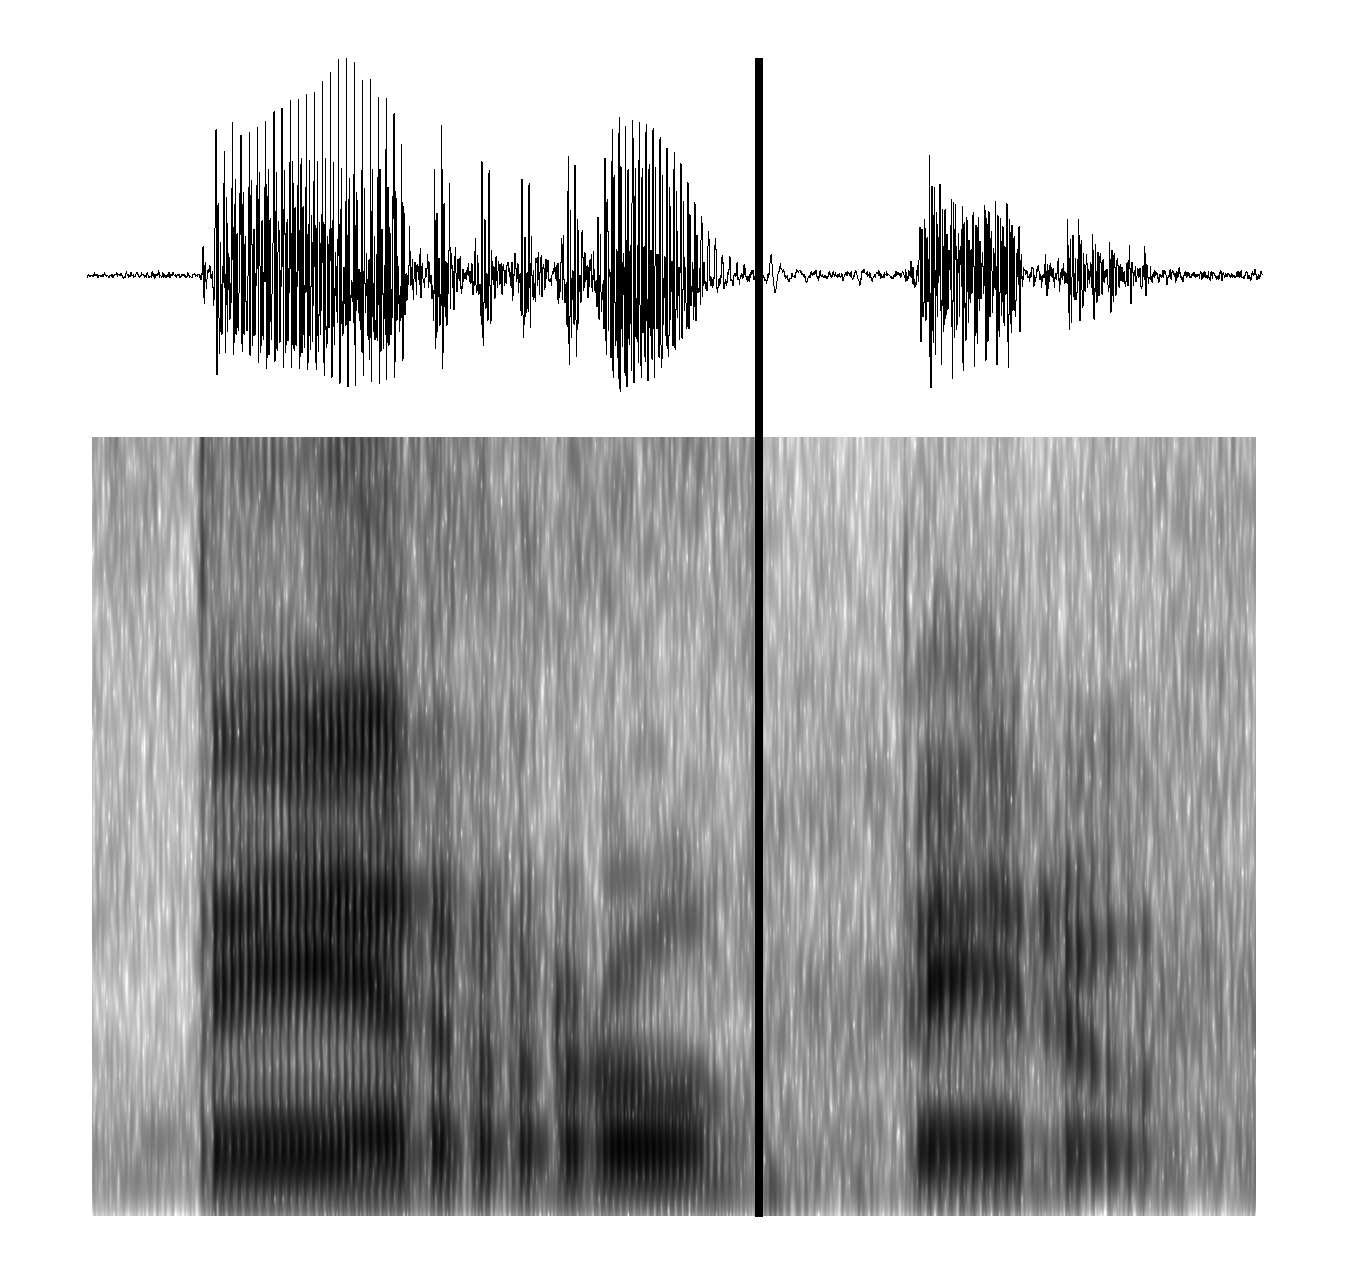
\includegraphics[width=1\linewidth]{rhotiques/images/praat_dogbut.pdf}
	\caption[Illustrations du /r/ et du /ɾ/ en espagnol]{À gauche : le trill dans le mot \textit{perro} /pero/ \textg{chien}. À droite : le tap dans le mot \textit{pero} /ɾ/ \textg{mais}. Les deux exemples sont issus de l'espagnol. Les deux mots ont été produits en isolation, et sont produits par deux locuteurs différents. Le premier (le trill) est produit par un locuteur de 25 ans de Meddelin Antioquia, Colombia, et le second (le tap) par un locuteur de 22 ans de Cartago Valle, Colombia. Le trill et le tap représentés ici sont considérés comme canoniques. L'oscillogramme est donné en haut, et le spectrogramme en bas (les axes sont manquants par choix).}
	\label{fig:praatdogbut}
\end{figure}

\subsection{Description du trill}

Cette sous-section du \textsc{trill} s'intéresse à ce segment d'un point de vue phonétique et phonologique.
Nous reprenons les différentes descriptions de ce segment qui peut impliquer un des trois articulateurs mobiles : les lèvres, la langue, ou l'uvule \parencite{ladefogedLateralsTrills1977}. Il faut souligner que dans cette thèse nous ne nous intéresserons pas aux trills bilabiaux impliquant la vibration des lèvres \parencite{rangelovBilabialTrillsAhamb2019} qui n'ont d'ailleurs jamais été inclus dans la catégorie des rhotiques \parencite{wieseRepresentationRhoticsRepresentation2011}. En ce qui concerne les trills uvulaires, ils sont abordés dans la \autoref{sec:similr} et dans le \autoref{chap:soundcompa}. \\

Nous nous focaliserons uniquement sur la vibration de la pointe de la langue qui donne lieu aux trills apicaux, en laissant de côté celle de la lame de la langue qui donne lieu aux trills laminaux.\\

Contrairement à la sous-section suivante sur le tap/flap, nous ne développerons pas l'origine du terme trill. Cependant, il est important de souligner que le terme peut être ambigu et refléter plusieurs réalités phonétiques de même que le symbole de l'Alphabet Phonétique International \textit{r} (ce point sera développé dans le \autoref{chap:jipa}).

\subsubsection{Acoustique et articulation du trill alvéolaire} \label{subsec:trill}

Le trill alvéolaire apical est un segment produit lorsque la pointe de la langue se maintient de manière lâche près de la crête alvéolaire, de sorte qu'un mouvement d'air fasse vibrer la pointe de la langue. Cela se traduit par des périodes où la langue touche la crête puis s'en sépare \parencite[318]{ladefogedCoursePhonetics2015}.
\textcite[49]{ladefogedLateralsTrills1977} suggèrent que peu de langues possèdent des trills, et que les trills de ces langues sont généralement alvéolaires. Les trills réalisés avec la pointe de la langue ont une fréquence de vibration moyenne de 28,6Hz $\pm$ 4,0.\footnote{\textcite{ladefogedLateralsTrills1977} trouvent que les trills produits avec d'autres articulateurs ont aussi une fréquence de vibration similaire ce qui peut expliquer un degré de similarité auditoire.} \textcite{lindauStory1985} obtient une fréquence de 25Hz sur son échantillon multilingue (soit 1 cycle toutes les 40ms) avec généralement deux à trois périodes. Le nombre de périodes dépend de différents facteurs
\footnote{Certains des facteurs sont développés en \autoref{subsec:trill_tap}.} qui peuvent être linguistiques (le contexte phonologique, la position dans le mot, l'accentuation de la syllabe, le nombre de syllabes du mot, la catégorie grammaticale) \parencite[cf. tableau p. 23 pour les études d'intérêt]{zahlerVariationistAccountTrill2014} et non-linguistiques (le sexe, l'âge [notons que les effets de l'âge et du sexe ne sont pas les mêmes en fonction des études], la classe sociale, le lieu de vie, les croyances, la densité du réseau social des locuteurs, ou encore le style de tâche effectuée pour la récolte de données) \parencite[cf. tableau p. 21-22 pour les études d'intérêt]{zahlerVariationistAccountTrill2014}.\\

Ainsi le trill est souvent caractérisé par la présence d'au moins deux périodes visibles au niveau du signal acoustique (\autoref{fig:praatdogbut}). Chaque période est composée d'une phase de contact (similaire à une obstruction; nous emploierons le terme de \textg{contact} ou d'\textg{obstruction} dans la suite de cette thèse) et une période de relâchement. Le trill à une période reste néanmoins possible, son articulation étant différente du tap/flap \parencite{spajicTrillsToda1996}.

\begin{displayquote}
	\textrm{[...]} even in cases where there is only a single contact with the roof of the mouth, the action is physiologically (but perhaps not auditorily) quite distinct from that of a tap. \parencite[p.50]{ladefogedPreliminariesLinguisticPhonetics1971}
\end{displayquote}


De plus, le trill est caractérisé par des prérequis aérodynamiques fins. \textcite{soleAerodynamicCharacteristicsTrills2002} cherche des tendances universelles dans le comportement des trills. L'autrice montre qu'en cas de manquement des pré-requis aérodynamiques, le segment ne sera pas trillé et/ou dévoisé (le tap est différent de nature et n'a pas de tels prérequis cf. \autoref{subsec:acous_tap_flap}).
En outre, \textcite{mcgowanTongueTipTrills1992} montre que la position de la langue, sa forme et son élasticité, ainsi qu'une différence de pression de part et d'autre de la constriction de la pointe de la langue, jouent un rôle dans l'initiation de la vibration.
\textcite{dhananjayaAcousticAnalysisTrill2012} suggèrent que triller entraîne une géométrie du tract oral qui change rapidement, ce qui rend les trills moins directs à étudier.
Ce sont les différents prérequis du trill qui en font un segment complexe et un des derniers acquis dans les langues du monde \parencite{mcleodChildrenConsonantAcquisition2018}.\\

Il n'existe pas à notre connaissance d'autres études sur la perception du trill, et de la discrimination de contraste de longueur, au sein d'une même langue autre que celle de \textcite{raymondInitialMedialGeminate2005}. Cette étude sur l'arop-lopek \glotto{arop1243}, langue parlée en Papouasie-Nouvelle-Guinée par quelques 3000 locuteurs/trices, s'intéresse au contraste entre le /r/ et le /rr/, la contrepartie géminée du /r/. Le flap [ɾ] est aussi présent dans la langue comme allophone intervocalique du /d/.
Trois études sont incluses dans l'article.
La première étude se focalise sur la production des trills et s'intéresse au nombre minimum, moyen et maximum de contacts que les trills et les trills géminées peuvent avoir.
La deuxième étude cherche à savoir si les locuteurs sont capables de discriminer, faire la différence entre un trill géminé et un trill non géminé. 
Finalement, la dernière étude se concentre sur la compréhension de la frontière de perception entre un trill et un trill géminé.\\

\textcite{raymondInitialMedialGeminate2005} ont enregistré six locuteurs mâles pour leur étude de production lors d'une tâche de lecture de liste de mots. Les trills en position intervocalique et finale pouvaient avoir au minimum un contact (88/364) ce qui n'était pas le cas lorsqu'ils étaient en position initiale (0/131). Certains trills géminés étaient aussi produits avec un contact, bien que ce n'était pas les productions les plus fréquentes (5 occurrences sur 218). Les trills en position initiale sont plus longs que les trills dans les autres positions.
Les trills ont été produits avec maximum 5 contacts, alors que les trills géminés ont été produits avec maximum 7 contacts.
Les trills géminés sont produits avec plus de contacts (en moyenne 3,76 contacts) que les trills non géminés (en moyenne 2,29 contacts).
L'étude de discrimination sur le terrain a permis de mettre en avant que les locuteurs sont capables de discriminer correctement un trill d'un trill géminé en position initiale et intervocalique. L'étude de perception sert à montrer qu'à partir de trills modifiés artificiellement, les locuteurs catégorisent dans les trills, les items avec moins de contacts, et dans les trills géminés, ceux avec le plus de contacts. De même que pour l'étude en production, une asymétrie existe entre les items en position initiale et ceux en position intervocalique. En position initiale, il faut plus de contacts pour qu'un item soit considéré comme un trill géminé.\\

La position en début de mot est favorable aux trills. Cependant, les rhotiques ont tendance a être défavorisées en initiale de mot à travers les langues \parencite{labruneWordinitialRhoticAvoidance2021}. Ces résultats sont néanmoins à mettre en contraste avec \textcite{kavitskayaTrillsPalatalizationConsequences2009} qui, sur la base de données du russe, montrent que le trill est défavorisé en position intervocalique. Cela permettrait d'expliquer les distributions des différents allophones des rhotiques cross-linguistiquement.\\


Les trills sont souvent étudiés par rapport à des langues indo-européennes, à l'exception de quelques études typologiques.
L'étude de \textcite{raymondInitialMedialGeminate2005} est intéressante car elle apporte de la phonologie de laboratoire sur le terrain avec une expérience de production, de discrimination et de perception. De plus, elle s'intéresse à une langue sous-étudiée (sur \href{https://www.google.com/maps/place/Matafum,+Papouasie-Nouvelle-Guin\%C3\%A9e/@-5.2182111,146.4002482,9.13z/data=!4m13!1m7!3m6!1s0x68f3e3520a551b3f:0x58a83294038393a4!2sLong+Island!3b1!8m2!3d-5.3535839!4d147.1464245!3m4!1s0x68f3fd93309894d3:0x2df33848a2f3c3c0!8m2!3d-5.3707325!4d147.0343745}{Long Island} en Papouasie-Nouvelle-Guinée) dans une aire géographique et dans une famille linguistique (austronésienne) et permet d'apporter des éléments de réflexion sur le contraste que peuvent faire les langues entre trois sons \textg{simil-r} : le flap, le trill et le trill géminé.


\subsection{Description du tap et du flap}

Après avoir décrit les principales caractéristiques du trill, nous décrivons le tap et le flap. Nous avons pris le soin de développer cette sous-section sur le tap et le flap car \textg{
[t]he alveolar tap is a fairly understudied rhotic, and many aspects of its variation within and between speakers as well as across languages are not fully known \parencite[86]{cathcartArticulatoryVariationAlveolar2012}}. Tout d'abord nous aborderons l'historique des termes tap et flap avant de décrire articulatoirement et acoustiquement ces segments.

\subsubsection{Terminologie et historique du tap/flap}

\begin{figure}
	\centering
	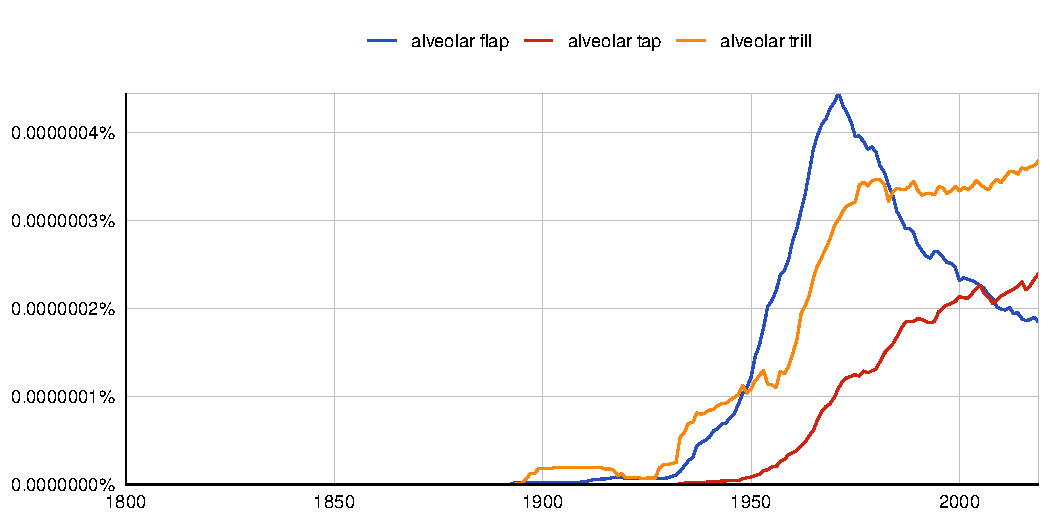
\includegraphics[width=1\linewidth]{images/google_ngram_trill_tap_flap}
	\caption[Google n-grams de \textg{alveolar trill}, \textg{alveolar tap}, \textg{alveolar flap}]{Fréquence des expressions \textg{alveolar trill}, \textg{alveolar tap}, \textg{alveolar flap} à partir des données de Google Books en utilisant le package \texttt{ngramr} sur \texttt{RStudio} \parencite{rcoreteamLanguageEnvironmentStatistical2020}, à partir du jeu de données de Google 2019.}
	\label{fig:googlengramtrilltapflap}
\end{figure}


On retrouve deux grandes approches concernant les taps et flaps. D'un côté, les études qui s'intéressent aux segments en prenant comme langue de référence l'anglais parlé aux États-Unis où le [ɾ] est un allophones des obstruentes /t, d/. De l'autre côté, il s'agit des études qui opposent le tap et le flap au trill car dans les langues étudiées on retrouve deux phonèmes /ɾ/ et /r/ comme en catalan. Il existe aussi une littérature moins abondante qui s'intéresse aux taps et flaps avec un point de vue utilisant d'autres langues.\\

Le \textg{trill} est apparu en premier, suivi du \textg{flap} puis du \textg{tap}. De la même manière, le symbole \textit{r} est apparu avant le \textit{ɾ} dans l'Alphabet Phonétique International. Nous avons fait le choix de garder le terme tap dans cette thèse comme terme générique pour parler des taps et des flaps. Nous justifions ce choix par l'éducation linguistique que nous avons reçue où le terme \textg{tap} était plus fréquent que le terme \textg{flap} reflétant leurs usages dans les publications scientifiques (Figure \ref{fig:googlengramtrilltapflap}). Le terme de flap est vraisemblablement d'abord apparu sur le continent européen où on le retrouve rapidement dans les publications de \textit{Le maître phonétique}. L'espagnol y était décrit avec un flap \parencite[8]{passySupplementAimPrincipales1904} et un trill. Le terme de tap, lui, est sûrement apparu sur le continent américain pour faire spécifiquement référence à l'allophone battu du /t/ et du /d/ produit en anglais américain entre deux voyelles. On retrouve dès les années 40 avec John Samuel Kenyon et Kenneth L. Pike l'apparition du terme \textg{tap}.

\begin{displayquote}
Voiced \textbf{t} is often described as a single-tap \textbf{r}. To the author's ear the two are quite distinct. Even when the voiced \textbf{t} has repeated taps (trilled  \textbf{t}) it is acoustically distinct from trilled \textbf{r} [...] \parencite[127]{kenyonAmericanPronunciation1943}
\end{displayquote}


\begin{displayquote}
In \textit{flap articulation} the articulator gives one rapid tap against its articulating region and then immediately releases; approach and release together are formed by a single ballistic movement. \parencite[124-125]{pikePhoneticsCriticalAnalysis1943}\
\end{displayquote}

En 1964, \citeauthor{ladefogedPhoneticStudyWest1968}\footnote{Nous n'avons pu consulter que la version de 1968.} publie un ouvrage sur les langues d'Afrique de l'ouest dans lequel il met en évidence que le hausa \glotto{haus1257} contraste entre un tap, qui peut être réalisé comme un trill, et un flap. Il s'agit de la première occurrence que nous avons trouvée où le tap est explicitement opposé au flap. Ses travaux lui permettront en \citeyear{ladefogedPreliminariesLinguisticPhonetics1971} de définir le tap comme un son où \textg{[o]ne articulator [is] thrown against another} et le flap comme un son où \textg{[o]ne articulator striking another one is passing} \parencite[46]{ladefogedPreliminariesLinguisticPhonetics1971}. Ces descriptions vont évoluer au fil des recherches menées sur les deux sons avec une influence sur le reste de la linguistique descriptive de terrain (comme nous le verrons avec les différences de terminologie dans le \autoref{chap:metagram}).

\begin{displayquote}
Alveolar tap ɾ also occurs in Hausa. Most of my informants used this sound, although occasionally it was replaced by a trilled r. Both these sounds occurred where Hausa orthography has r. There is also a contrasting sound which is sometimes written as r, and which appears to be a retroflex flap ɽ. [...] The nearest I can come to agreeing with this is to say that the first sound is a trill which has a statistical probability of consisting of only one tap. \parencite[30]{ladefogedPhoneticStudyWest1968}
\end{displayquote}

Cette section a servi à mettre en évidence que l'existence des deux termes tap et flap est historiquement justifiée. Les publications contemporaines font souvent le choix d'un terme ou de l'autre (ce qui n'est pas problématique, cela n'ayant pas de conséquences pour les analyses).\footnote{Par exemple, dans notre \autoref{chap:jipa} sur les \textit{Illustrations of the IPA} nous avait fait le choix (qui n'était pas vraiment éclairé au moment de l'écriture) d'utiliser le terme \textg{tap}.}

\subsection{Acoustique et articulation du tap/flap} \label{subsec:acous_tap_flap}

Nous détaillons dans cette sous-partie les différentes études qui ont eu comme objet de recherche le tap et/ou le flap.
\textcite[128]{catfordFundamentalProblemsPhonetics1977}, se basant sur les travaux de \textcite{ladefogedPhoneticStudyWest1968}, utilise le terme \textg{flap}. Le flap est articulatoirement décrit comme un son produit lorsqu'un organe articulatoire approche un autre (stationnaire) créant un contact momentané avant de se retirer (aussi connu sous le nom de \textg{one-tap r}). Deux types de flaps sont mis en avant en fonction de la mise en action de la langue. D'un côté, les flaps \textg{flick} [ɾ] sont produits lorsque l'articulateur revient à sa position de départ, et de l'autre, les flaps \textg{transient} [ɽ] sont produits lorsque l'articulateur mobile entre en contact momentané avec l'articulateur fixe dans son mouvement vers une position finale (Figure \ref{fig:figure29catford}). Les deux types de segments ont une durée comprise entre 10 et 30ms.\\

\begin{figure}
	\centering
	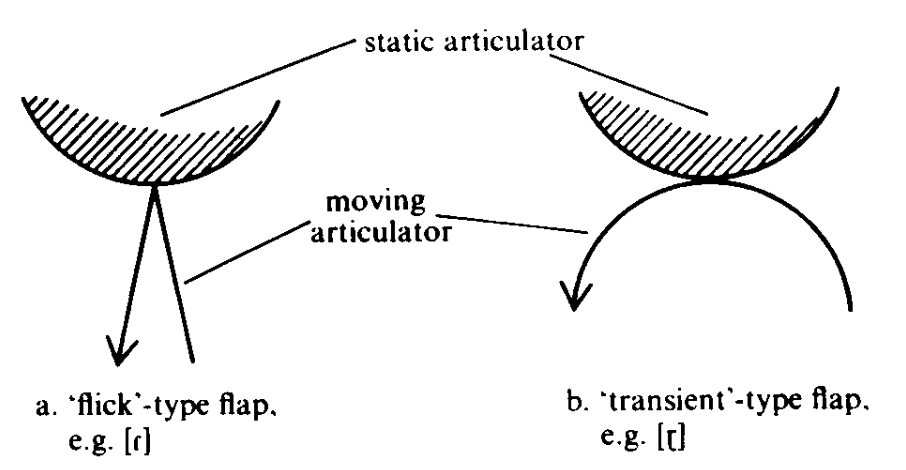
\includegraphics[width=0.9\linewidth]{rhotiques/images/figure_29_catford}
	\caption[Schématisation des \textg{flaps}. Figure issue de Catford (1977)]{Schématisation par \textcite[129]{catfordFundamentalProblemsPhonetics1977} des deux types de flaps identifiés. L'un sera généralement repris par la littérature comme un tap [ɾ], et l'autre comme un flap [ɽ].}
	\label{fig:figure29catford}
\end{figure}

\textcite[129]{catfordFundamentalProblemsPhonetics1977} souligne l'importance de la momentanéité des flaps, des mouvements balistiques, les opposant aux stops : \textg{a stop can be prolonged; a flap cannot be prolonged}.\footnote{\textcite[397]{newmanHausaLanguageEncyclopedic2000} mentionne qu'en hausa le flap géminé existe de même que le \textg{tap/roll} geminé. Le flap géminé se manifeste phonétiquement par une augmentation de la \textg{temporal period of the retroflex flap gesture}, là où le \textg{tap/roll} devient un trill discernable. \textcite[237]{ladefogedSoundsWorldLanguages1996}, en hausa, analysent la géminée du flap comme une longue approximante rétroflexe.} Contrairement aux stops, les flaps mettent en jeu une surface de contact moins importante selon \textcite[251]{catfordFundamentalProblemsPhonetics1977}.\\

En anglais américain, le flap peut être un allophone du /t/ et du /d/. Le flap est un des allophones des occlusives alvéolaires en position post-voyelle accentuée \parencite{zueAcousticStudyMedial1979}.
Avec des enregistrements de trois hommes et trois femmes, les auteurs analysent les données et soulignent la présence de variation dans les réalisations des flaps. En effet, la phase de \textg{closure} peut être plus ou moins complète. Lorsqu'elle est partielle, on peut retrouver au niveau du signal acoustique de la turbulence similaire à celle qu'on peut retrouver avec les fricatives voisées. Les auteurs mesurent en moyenne 27 ms pour les /d/ et 26 ms pour les /t/ avec un écart autour de la moyenne entre 10 ms et 40 ms, principalement dû au contexte vocalique. Une durée courte de flap indique un mouvement rapide de la langue montant et descendant de la pointe de la langue, alors qu'une durée longue est indicatrice d'une pression accumulée pendant la constriction de la langue qui s'accompagne d'un relâchement accompagné par une explosion de bruit visible sur le spectrogramme. Cela peut s'expliquer par la position du corps de la langue. S'il est bas, alors le mouvement de la pointe de la langue peut être bref, alors que s'il est haut, le mouvement de la pointe de la langue \textg{overshoot} la zone alvéolaire rendant l'occlusion plus longue.\\


\textcite{zengUnderstandingFlappingXiangxiang2007} s'intéresse aux flaps dans le dialecte chinois de Xiangxiang\footnote{Selon nous, il est regrettable que cette description allophonique ne soit pas présente dans l'\textit{Illustration of the IPA} publiée, disponible en FirstView (cf. \autoref{subsec:data_coll}) à propos du même dialecte du chinois \parencite{zengXiangxiangDialectChinese2020}. Nous nous interrogeons donc sur la proportion des langues décrites dans JIPA à avoir des occlusives qui sont réalisées comme des flaps dans certains contextes, mais qui ne sont pas décrites comme telles.} qui sont des allophones du /d/ et du /t$^\textrm{\tiny h}$/ en position intervocalique pré-syllabe accentuée et pré-syllabe non accentuée. L'étude se base sur quatre locuteurs et une locutrice et permet de mettre en évidence de la variation intra-individuelle. \citeauthor{zengUnderstandingFlappingXiangxiang2007} montre qu'il existe dans cette position pour le /d/ un continuum allant du [d] \textg{typique}, avec une occlusion longue et une barre d'explosion, au flap, avec une occlusion de courte durée et sans barre d'explosion. Dans ce continuum, on retrouve aussi le flap long avec une durée plus longue que le flap typique, et le [d] court avec une durée d'occlusion plus courte que celle du [d] typique.
Un dernier variant, considéré comme \textg{extrême} par \citeauthor{zengUnderstandingFlappingXiangxiang2007}, possède une structure similaire à celle d'une approximante, c'est-à-dire avec un degré moindre de constriction orale. Pour le /t$^\textrm{\tiny h}$/, cinq variants sont identifiés :

\begin{itemize}
\item le typique [t$^\textrm{\tiny h}$],
\item le typique [d$^\textrm{\tiny h}$],
\item le court [d$^\textrm{\tiny h}$],
\item le flap aspiré long
\item et le flap aspiré typique.
\end{itemize} 

Des données aérodynamiques sont aussi incluses et permettent de montrer une relation entre le flux d'air oral et les différents motifs acoustiques.
Ainsi, \textcite{zengUnderstandingFlappingXiangxiang2007} montre que le processus de \textg{flapping} n'est pas binaire. L'accentuation de la voyelle précédente est exclue comme facteur explicatif des différents variants mais les voyelles précédentes et suivantes permettent d'expliquer la variation à cause de co-articulation.\\

\textcite{sonPitfallsSpectrogramReadings2008}, dans la continuité de \textcite{zengUnderstandingFlappingXiangxiang2007}, s'intéresse au flap allophone de la liquide /l/ en coréen. Son étude inclut des données acoustiques de deux locutrices native de Séoul en plus de mesures articulométriques. \citeauthor{sonPitfallsSpectrogramReadings2008} met en évidence de la variation intra-individuelle avec cinq variants :

\begin{itemize}
	\item Flap voisé avec explosion
	\item Flap voisé sans explosion
	\item Flap partiellement voisé avec explosion
	\item Flap non voisé avec explosion
	\item Flap \textg{extrême} (reprenant la description de \textcite{zengUnderstandingFlappingXiangxiang2007})
\end{itemize}

L'étude articulatoire a permis de montrer que, même lorsqu'il n'y avait pas de constriction dans le cas des flaps extrêmes, il y avait quand même un mouvement large de la pointe de la langue, mettant en évidence une certaine invariance dans l'articulation du flap. Cette invariance est donc à mettre en contraste avec la variation dans les résultats des études acoustiques.\\

Les travaux initiés par Derrick, Gick et leurs collègues \parencite{derrickQuantitativeAnalysisSubphonemic2008,derrickTwoPhonologicalSegments2010,derrickIndividualVariationEnglish2011,derrickAcousticCorrelatesFlaps2013} sur la base d'ultrasons ont permis de mettre en avant la variation dans les mouvement associés au processus de \textg{flapping} en anglais américain. On retrouve quatre variants (Figure \ref{fig:tapflap}):

\begin{itemize}
	\item Up-flap
	\item Down-flap
	\item Alveolar tap - le tap alvéolaire
	\item Postalveolar tap - le tap post-alvéolaire
\end{itemize} 

La catégorisation des différents variants s'est faite en fonction du mouvement de la pointe de la langue, ainsi que de sa direction. Les travaux préliminaires de \textcite{derrickQuantitativeAnalysisSubphonemic2008} montrent que tous les participants produisent les quatre variants et que la variation est influencée par la position de la langue avant et après le segment \parencite{derrickTwoPhonologicalSegments2010}. \textcite{derrickIndividualVariationEnglish2011}, en étudiant huit locutrices et dix locuteurs, obtiennent que trois participants n'ont pas produit un des variants (le tap post-alvéolaire). Ainsi, les auteurs montrent que les réalisations \textg{flap} sont plus fréquentes que les réalisations \textg{tap}. On retrouve en plus de la variation non-conditionnée puisque pour les mêmes mots, certains participants ont utilisé différentes stratégies articulatoires. \\

\begin{figure}
	\centering
	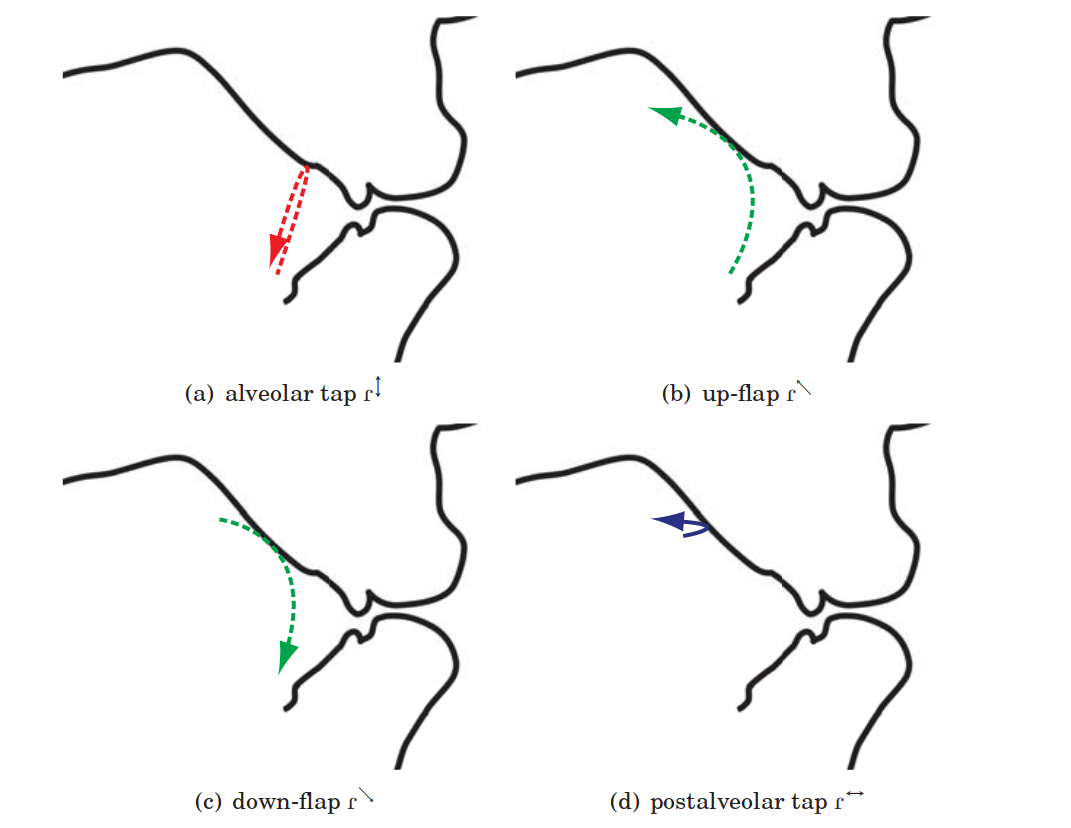
\includegraphics[width=0.7\linewidth]{rhotiques/images/tap_flap}
	\caption[Différents mouvements pour le tap/flap en anglais américain. Figure issue de \textcite{derrickAcousticCorrelatesFlaps2013}]{Les différents mouvements pour le tap/flap en anglais américain. La figure est issue de \textcite{derrickAcousticCorrelatesFlaps2013}. Les différents mouvements ont été obtenus par ultrason.}
	\label{fig:tapflap}
\end{figure}

\textcite{derrickIndividualVariationEnglish2011} offrent un nouveau regard sur les données de différentes langues. Pour eux, les contrastes entre les quatre différents variants du flap sont possibles. Ils mettent en avant des contrastes phonétiques sur la base de contrastes entre tap et flap, comme c'est le cas pour le punjabi\footnote{Il existe une \textit{Illustration of the IPA} pour le punjabi \parencite{hussainPunjabiLyallpuriVariety2019} où les auteurs mentionnent un contraste entre deux rhotiques : un tap alvéolaire /ɾ/ et un tap rétroflexe /ɽ/ (\textg{retroflex tap} [\textit{sic}] (p. 6). Les auteurs illustrent une paire minimale et explicitent que la consonne rétroflexe met en avant un abaissement précoce des troisième et quatrième formants.} \parencite[645]{shacklePanjabi2003}, ou le norvégien où l'on retrouve un [ɾ] s'opposant à un [ɽ] dans certains dialectes \parencite[24]{kristoffersenPhonologyNorwegian2000}.\\

L'étude préliminaire de 2013 de \citeauthor{derrickAcousticCorrelatesFlaps2013} s'intéresse à l'acoustique des quatre variants. Les auteurs montrent qu'il y a des différences significatives pour la fréquence fondamentale et les cinq premiers formants entre les variants. Des deux premiers formants, les auteurs concluent que les quatre variants ont des configurations différentes en termes d'aperture et de postériorité, mais que ces différences se réduisent après la consonne. En ce qui concerne le troisième formant, les auteurs concluent que les variants ont différents points de contact. Le down flap a son point de contact le plus proche des dents, suivi du tap alvéolaire et du up flap, et c'est le tap post-alvéolaire qui a son point de contact le plus haut.\\

Dans certains cas, le tap/flap n'est pas considéré comme un allophone d'un stop mais d'une rhotique, c'est le cas de l'espagnol ou du catalan où le tap a été étudié en opposition à une autre rhotique de ces langues : le trill. Nous avons détaillé les études sur le trill en \autoref{subsec:trill} et nous faisons le lien entre les deux segments en \autoref{subsec:trill_tap}. Dans cette section, nous ne parlerons que du tap/flap.

\textcite{recasensProductionCharacteristicsApicoalveolar1991} étudie de manière préliminaire les caractéristiques de production du tap apico-alvéolaire en catalan avec l'électropalatographie sur la base de ses propres productions.
L'occlusion n'est pas systématiquement complète pour le tap. Il y a plus de contact pour le tap lorsqu'il est précédé et suivi par une voyelle postérieure [a, u] que lorsqu'il est précédé et suivi par une voyelle antérieure [i]. Ce manque de contact associé à la voyelle antérieure [i] suggère, selon \citeauthor{recasensProductionCharacteristicsApicoalveolar1991}, qu'il peut exister une incompatibilité entre la constriction de la pointe de la langue et l'élévation du dos de la langue. Ses résultats lui permettent aussi de supposer que la position du corps de la langue ne nécessite pas tant de contrôle articulatoire, à cause de la présence de coarticulation avec le contexte vocalique. L'étude de \textcite{recasensStudyLightDAC1999}, avec plus de participants, vient confirmer les résultats de l'étude préliminaire. Les deux études mettent principalement en avant les différences en terme de coarticulation entre le trill et le tap plutôt que de caractériser finement le tap.

\begin{displayquote}
	The tap is articulated with a restricted short apicoalveolar closure and more predorsum lowering than other alveolars. In comparison with /n/, /ɾ/ involves less apico-predorsal coupling and exhibits larger dorsopalatal and F2 troughs in the sequence /iCi/. \parencite[163]{recasensStudyLightDAC1999}
\end{displayquote}

Des études dans d'autres langues soutiennent également l'appartenance du tap et du flap dans la catégorie des rhotiques. Par exemple, \textcite[96]{carvalhoEstruturasFoneticasLingua2010} effectue une analyse acoustique préliminaire du flap en tikuna où il est considéré comme une rhotique. \citeauthor{carvalhoEstruturasFoneticasLingua2010} obtient de la variation inter-individuelle  mais aussi intra-individuelle avec un continuum allant de l'occlusion brève mais complète à l'approximante. Des quatre locuteurs enregistrés, un a présenté des occurrences avec systématiquement une constriction, un a systématiquement produit des flaps sans constriction, et deux ont produit un mélange des différents variants. Toutes les productions de flaps étaient voisées et avaient une durée moyenne de 21 ms. \textcite{savuMoreRhoticTap2014} s'intéresse au tap en macédonien et en roumain en mettant en évidence les différences de perceptions entre les locuteurs des deux langues.\\

Pour étudier la rhotique du grec, \textcite{baltazaniManyFaces2013} combinent une étude articulatoire et acoustique. La rhotique a été généralement décrite comme un tap en position intervocalique. Les résultats de l'étude confirme que la rhotique est très majoritairement produite avec un contact court dont la durée varie entre 11 et 57 ms, ce que les auteurs interprètent comme un tap. Des trills sont aussi retrouvés parmi les productions. Le degré de constriction est variable car influencé par plusieurs facteurs. Des différentes expériences menées, plus de 50\% des occurrences sont produites avec une constriction incomplète. Ce contact incomplet se retrouve notamment lorsque les taps ne sont pas produits dans un groupe consonantique. De même, le contact incomplet se retrouve plus dans les syllabes hétérosyllabiques ainsi qu'en position initiale de mot ou lorsque le segment est adjacent à une fricative (en opposition à un stop). De plus, les auteurs mettent en avant l'importance d'un élément vocalique pour le mouvement du tap.

%Parmi les éléments acoustiques qui caractérisent le rabat en tant que "segment acoustique" (cf. Fant 1973 ; Recasens 1991b ; Ting 2007 ; Son 2008) figurent les suivants :
%(1) durée de la discontinuité spectrographique introduite par le geste d'occlusion ;
%(2) l'intensité de la discontinuité (caractérisant une occlusion complète ou une zone plus large au point de contrition) ;
%(3) le modèle de transition des formants dans les voyelles voisines ;
%(4) présence ou absence de voisement ;
%(5) présence ou absence de formants pendant la discontinuité ou l'occlusion.






\section{Distribution et variation cross-linguistique des sons \textg{simil-\textit{r}}}

\subsection{Distribution dans le monde}

Deux travaux d'importance ont eu comme objectif d'étudier la variation dans les trills avec une approche typologique (avec un recours minimal à des bases de données existantes). Paradoxalement, bien que le thème de ces travaux soit directement relié au contenu de cette thèse, nous n'avons pas eu d'accès direct aux ouvrages à l'exception de \textcite{lindauStory1985}.
Nous allons tout d'abord détailler le manuscript non publié de Jones\footnote{Jones, M. (unpublished). Patterns of variability in apical trills: An acoustic study of data from 19 languages.} puis la thèse de \textcite{inouyeTrillsTapsStops1995} et finalement les travaux de \textcite{lindauStory1985}.\\

Pour cela, nous avons fait le choix de rapporter ces travaux à travers leurs citations dans la littérature. Comme il s'agit de travaux qui étudient plusieurs langues en même temps, nous pouvons supposer que la même méthodologie a été utilisée pour étudier les langues, et donc dans une certaine mesure contrôler la variation entre les productions.\\

\textcite[23]{punnooseAuditoryAcousticStudy2010} mentionne que Jones considère le trill comme central dans les rhotiques, bien que cela puisse amener à l'interprétation fausse qu'une langue avec un /r/ trillé le réalise forcément comme un trill [r]. Jones met en avant de la variabilité dans son étude sur 19 langues due à la complexité articulatoire du segment\footnote{Les différents aspects qui font du trill un segment complexe sont abordés en \autoref{subsec:trill} et dans le \autoref{chap:jipa}}. Les 19 langues utilisées possèdent une seule rhotique. Jones s'intéresse aux rhotiques dans des listes de mots mais aussi dans des histoires \textg{narratives} récoltées en laboratoire. Ses résultats (p. 23 dans \textcite{punnooseAuditoryAcousticStudy2010}) montrent que le trill n'est réalisé comme tel que dans un tiers des cas avec généralement deux occlusions. Les trills sont moins fréquents dans les narratives que dans les listes de mots, et également plus fréquents dans des contextes consonantiques qu'en position intervocalique avec le contexte post-vocalique pré-consonantique favorisé.
Acoustiquement, \textcite[24]{punnooseAuditoryAcousticStudy2010} explique les résultats de Jones par la présence d'un deuxième contact des trills, généralement affaibli. Cela peut se traduire par un manque de détection de la part d'études acoustiques. Enfin, cela donne du crédit à l'hypothèse que ce genre de trill cause une réanalyse perceptuelle menant à un changement du trill au tap. Cependant, pour Jones il existe aussi des réalisations non trillées qui sont des taps. Il ne peut pas affirmer que ces taps soient qualitativement différents des \textg{one-contact trill} (p. 24).\\

Du résumé de la thèse de \textcite{inouyeTrillsTapsStops1995}, nous pouvons dire que l'autrice s'est intéressée à la relation entre trills, taps et stops. L'originalité de sa thèse est d'avoir travaillé sur quelques 65 familles de langues, et d'y avoir inclus des données phonétiques d'environ une quinzaine de langues. Ces données sont des données de première main mais aussi de bases de données déjà existantes (au moins pour les langues australiennes incluses et celles provenant de UCLA phonetic database). L'autrice montre dans sa thèse que les taps comme allophones intervocaliques d'occlusives sont fréquents dans les langues du monde, de même que l'allophone tap en position intervocalique dans les langues décrites avec un trill.\\

\textit{The Story of /r/} de \textcite{lindauStory1985} cherche ce qui caractérise les rhotiques. Pour ce faire, sans détailler sa méthodologie, l'autrice utilise les productions de 92 locuteurs/trices issus de plus de 13 langues/dialectes dont 9 avec un trill [r] comme allophone. Ses données lui permettent de comparer les trills alvéolaires et les trills uvulaires  et d'en dégager les tendances acoustiques. Ses mesures du troisième pic spectal (le troisième formant F3) suggèrent que les productions des trills sont variables chez des locuteurs/trices qui produisent des segments avec un lieu d'articulation plus ou moins alvéolaire, ou plus ou moins dental (de même \textcite{dhananjayaAcousticAnalysisTrill2012} montrent que les trills sont flexibles quant à la position du dos de la langue). La contribution la plus importante de \citeauthor{lindauStory1985} utile à notre thèse est d'affirmer que la réalisation du /r/ comme consonne trillée n'est pas commune même lorsque ces sons ont été décrits comme étant des \textg{trills} (p. 161). En effet, d'autres réalisations sont possibles comme des taps ou des approximantes. \citeauthor{lindauStory1985} met ainsi en avant de la variation à la fois entre les individus (variation inter-individuelle) et au sein des productions des mêmes individus (variation intra-individuelle), qui ne sont pas toutes trillées (sauf pour l'espagnol\footnote{Bien que peu d'occurences de trills en espagnol sont incluses dans notre analyse acoustique, nous retrouvons aussi cette tendance dans le \autoref{chap:acoustics}}).\\
	

\subsection{Exemples de la variation en français et en espagnol autour du monde}

Nous montrons que la variation n'est pas seulement inter-langues mais peut aussi se retrouver au sein de langues parlées à plusieurs endroits du globe avec un héritage colonial. C'est le cas du français et de l'espagnol que nous illustrons dans les sous-sections suivantes.

\subsubsection{Les productions du /r/ dans la francophonie}

Le /r/ français n'est pas uniquement articulé comme une fricative ou une approximante alvéolaire. Ainsi, dans certaines régions du monde francophone il est encore possible de trouver des réalisations de la rhotique alvéolaire. En ce qui concerne les productions uvulaires, elles sont, de même que pour les rhotiques alvéolaires, maîtrisées tardivement par les enfants \parencite{dossantosDeveloppementPhonologiqueFrancais2007,metralCaracterisationAcoustiqueRhotique2021}.\\

Le français s'est exporté dans différentes régions du monde, entraînant des changements spécifiques à chaque région où il a été nouvellement parlé. De manière générale, on retrouve une tendance pour la rhotique apicale à laisser place à la rhotique uvulaire. \textcite{thibaultFrenchOutsideEurope2022} nous résume les différentes études mettant en évidence les variations dans les sons du français en fonction des différentes ères coloniales. Nous présentons les aires géographiques avec les différentes réalisations dans l'ordre donné par \citeauthor{thibaultFrenchOutsideEurope2022}. La variation n'est pas détaillée, avec dans la plupart des cas un ou deux allophones majoritaires décrits à travers leur symbole de l'API.\\

Le français de Saint-Laurent utilise un [r] apical qui est en cours de changement en faveur du [ʁ] uvulaire, de même qu'en français de Montréal \parencite{sankoffInstabilityAlternationMontreal2013,morinApicalUvularWhat2013}.
Le français acadien utilise le flap [ɾ]. Similairement, on retrouve le flap [ɾ] dans le français de Louisiane. À Haïti, en Guadeloupe ou en Martinique, on retrouve différents allophones dont les fricatives [ɣ] vélaire et [ʁ] uvulaire ainsi que l'approximante [w].
Dans les îles de l'océan Indien, en Mauritanie le /r/ est soit supprimé, soit produit uvulairement avec peu d'intensité \parencite[263--264]{ledegenFrenchMauritiusSpeaker2016}.
Au Maghreb, la rhotique a été produite comme un trill alvéolaire [r] mais un changement est en cours et elle est principalement produite comme le [ʁ] uvulaire\footnote{\textcite{thibaultFrenchOutsideEurope2022} référant à Morsly (2003, p. 937) ne mentionne que les productions des hommes sans expliciter ce que les femmes produisent.} Ce changement de la production alvéolaire à l'uvulaire est aussi présent au Liban où les locuteurs jeunes et cultivés préfèrent le [ʁ] uvulaire parisien \parencite[25]{thibaultFrenchOutsideEurope2022}. En Afrique subsaharienne, on retrouve le [r]. 
Dans le français du Djibouti, le flap [ɾ] est présent, dans celui de Madagascar, il s'agit d'un trill [r]\footnote{De même que pour le /r/ du Maghreb, \textcite{thibaultFrenchOutsideEurope2022} réfère à Bavoux (1993, pp. 181-183) pour insister sur le fait que la variante est principalement présente chez les hommes.}. 
Finalement, dans le Pacifique, à Tahiti, le /r/ est réalisé comme un flap alvéolaire ou trill [r].

\subsubsection{Les productions du /r/ dans le monde hispanique}

De même que le français, l'espagnol s'est exporté à l'international.
L'espagnol est parlé principalement en Espagne et en Amérique latine. Semblablement au français, l'espagnol de l'Amérique Latine a été en contact et influencé par de nombreuses langues, notamment des langues locales et des langues parlées par les esclaves venus d'Afrique.\\
%~\\
%/rr/\\
%Fricative pronunciation : Page 12, 31, 81, 138, 140, 171, 189-90, 200, 209, 222-4, 248, 265, 272, 279, 308, 319, 322\\
%Velarizeed pronunciation : 140-1, 333-4\\
%~\\
%/r/\\
%assibilation: 12, 22, 25, 81, 171, 189-90, 200, 209, 22-4, 248, 265, 280, 308, 319, 322\\
%neutralization with /l/: 10-12, 23, 25, 98, 126-8, 139, 168, 187, 200, 211-12, 231-2, 239-40, 271, 283, 299, 322-3, 350
%/tr/\\
%~\\

%Lipski 1991c
%Nunez Cedeno 1990

L'espagnol d'Argentine est caractérisé par un phonème /rr/\footnote{Pour certains auteurs, le /rr/ fait référence à un trill et le /r/ a un tap. C'est le cas ici.} réalisé comme un trill alvéolaire dans le littoral du sud incluant Buenos Aires (p. 170). Au nord, l'espagnol est influencé par les langues locales.
À l'est, l'influence du guarani entraîne une réalisation de type \textg{groove fricative} pour le phonème. Mais dans certains lieux près de la frontière avec le Paraguay, ce dernier est réalisé comme un [ž] (p. 171).
Dans le nord-ouest, le quechua influence l'espagnol mais \textcite{lipski1994latin} ne précise pas les réalisations. \citeauthor{lipski1994latin} ne donne pas d'indications pour l'espagnol de l'Uruguay.\\

En Bolivie, dans les \textg{Altiplano highlands}, le /rr/ est réalisé comme une \textg{groove fricative} ou sibilante qui peut être alvéo-dentale ou prépalatale (p. 189). Le trill [ř] décrit par Gordon\footnote{Gordon Alan (1987) Distribucion demografica de los alofonos de /rr/ en Bolivia. Actas del I congreso International sobre el espanol de America.} (1987, cité par \citeauthor{lipski1994latin}) commence cependant à se généraliser. Dans les \textg{Lowland Llanos}, l'assibilation du /rr/ n'est pas présente bien qu'une tendance aille dans ce sens (Gordon (1987) cité par \citeauthor{lipski1994latin}). Au Chili, l'espagnol est influencé par le mapuche (mapudugnun) (cf. \autoref{subsec:mapuche}) et le /rr/ y est produit comme une \textg{groove fricative}. Au Paraguay, on retrouve une réalisation de trill alvéolaire pour le /rr/ \parencite[308]{lipski1994latin}.\\

En fonction des régions de Colombie, on retrouve différentes influences liées à l'esclavagisme et aux minorités indigènes. Dans les \textg{central highlands}, le /rr/ est un trill faible, avec des réalisations parfois \textg{groove fricatives} là où l'espagnol est influencé par le quechua \parencite[209]{lipski1994latin}. Pour les autres parties de la Colombie, \citeauthor{lipski1994latin} ne donne pas d'indications.
Le quechua a aussi influencé l'espagnol de l'Équateur. Le /rr/ est réalisé comme un trill alvéolaire sauf dans la région \textg{Central highlands}, où il s'agit d'une \textg{groove fricative} similaire à [ž], et dans la région de Cañar et Azuay, où il s'agit d'une fricative \parencite[247--9]{lipski1994latin}. Au Pérou, on retrouve au sud une fricative similaire au [ž], et au nord de la région Andine, c'est le trill qui prédomine similairement à celui du sud de l'Équateur \parencite[320]{lipski1994latin}.
Au Venezuela, on retrouve un trill alvéolaire pour le /rr/ qui peut être partiellement dévoisé \parencite[350]{lipski1994latin}\\

L'espagnol du Costa Rica est constitué de plusieurs dialectes. Dans la \textg{Central Valley}, le /rr/ est caractérisé par une \textg{groove fricative} [ž] qui peut devenir une rétroflexe en locution rapide \parencite[222]{lipski1994latin}. Dans les autres dialectes, on retrouve des fricatives ou sibilantes \parencite[224]{lipski1994latin}. \citeauthor{lipski1994latin} ne donne pas d'indications pour l'espagnol du Salvador et celui du Panama. L'espagnol du Guatemala possède un /rr/ réalisé comme une fricative qui varie d'une fricative prépalatale [ž] à une fricative rétroflexe. Pour le Honduras, les locuteurs éduqués de Tegucigalpa produisent une \textg{groove fricative} pour le /rr/. Au Mexique, on retrouve des influences des langues maya. Le /rr/ y est réalisé comme un trill alvéolaire. La \textg{groove fricative} se retrouve dans le parler des femmes de classe moyenne où la réalisation est vue comme prestigieuse (p. 279). A Chiapas, on retrouve une sibilante comme /rr/. Au Nicaragua, sur la côte, on peut retrouver le /rr/ produit comme un flap ou comme une approximante rétroflexe \parencite[291]{lipski1994latin}. 
À Cuba, l'espagnol a été influencé par les langues parlées par les esclaves d'Afrique. On y retrouve un trill dévoisé pour le /rr/ et une vélarisation possible pour les strates sociales basses \parencite[231]{lipski1994latin}. De même, le trill dévoisé est présent dans l'espagnol de République Dominicaine \parencite[239]{lipski1994latin}. À Puerto Rico, des /rr/ 'vélarisés' sont présents. Il s'agit de productions allant du [x] ou [ʀ] \parencite[333]{lipski1994latin} avec une influence possible soit du français, soit de langues d'Afrique de l'ouest.\\

Cette partie a servi à illustrer la complexité de la réalisation du /r/ et du contact de langue. Ce qui est considéré comme un trill n'est pas forcément trillé car beaucoup de facteurs peuvent intervenir. De même que les langues coloniales ont été influencées par les langues natives, les langues natives peuvent aussi être influencées par les langues coloniales (cf. \autoref{subsec:mapuche}). Le transfert du trill n'est pas que vertical, c'est-à-dire depuis une langue mère vers une langue fille, mais peut aussi être horizontal, c'est-à-dire entre différentes langues. Il s'agit d'un point important à mentionner mais pas crucial pour cette thèse.



%\input{rhotiques/candidats}

\section{Pourquoi faut-il s'intéresser au \textg{trill} ?}

\begin{displayquote}
	The statistical dominance, and in fact prototypical status, of the alveolar trill among the rhotics is in striking contrast to the considerable difficulties it seems to raise for articulation. \parencite[4]{wieseRepresentationRhoticsRepresentation2011}
\end{displayquote}

C'est sur cette citation de \citeauthor{wieseRepresentationRhoticsRepresentation2011} que nous commençons à exprimer notre intérêt pour le trill. Il s'agit d'un segment complexe à produire, mais qui pourtant est présent dans de nombreuses langues. De plus, ce segment varie entre les locuteurs mais aussi entre les langues. Sa représentation est omniprésente dans les transcriptions en dépit d'autres symboles généralement plus précis acoustiquement.\\

Ce sont plein de facteurs qui rendent l'étude du trill compliquée, voire complexe. Il faut osciller entre phonétique et phonologie, être capable d'avoir une vision globale du phénomène tout en appréciant les détails.
Pour cela, nous souhaitons comprendre sa distribution et en établir une typologie pour comprendre dans quelle mesure sa production est arbitraire. Enfin, nous espérons qu'une meilleure appréhension du trill permettra de mieux comprendre pourquoi certaines personnes ne peuvent pas produire ce son.

